% General recursive call tree schematic for the L3c lecture (Understanding
% Recursion section). Symbolic companion to Fig-Fibonacci-Recursive.svg, which
% shows the concrete n = 4 instance in the example notebook.
%
% Build (from this directory):
%   pdflatex Fig-Recursion-Call-Tree.tex
%   pdf2svg Fig-Recursion-Call-Tree.pdf Fig-Recursion-Call-Tree.svg
\documentclass[tikz,border=8pt]{standalone}
\usetikzlibrary{arrows.meta}
\definecolor{chemered}{HTML}{EF4035}
\definecolor{chemewheat}{HTML}{FAEEE2}
\begin{document}
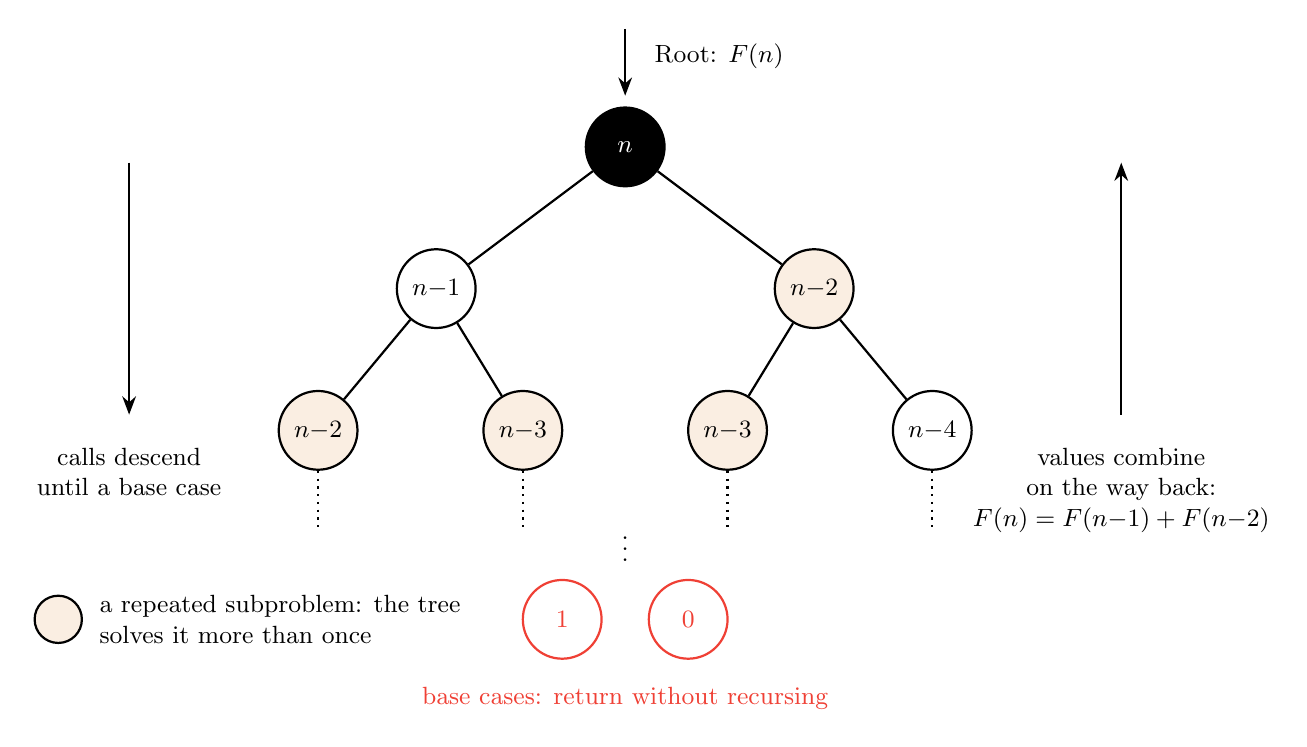
\begin{tikzpicture}[
    call/.style={circle, draw=black, thick, minimum size=10mm, inner sep=1pt, font=\small},
    dup/.style={call, fill=chemewheat},
    base/.style={call, draw=chemered, text=chemered},
    note/.style={font=\small, align=center},
    link/.style={thick},
    x=1cm, y=1cm]

    % ----- the call tree: node labels are the argument of F, as in the n = 4 figure
    \node[call, fill=black, text=white] (root) at (0, 0) {$n$};
    \node[call] (l)  at (-2.4, -1.8) {$n{-}1$};
    \node[dup]  (r)  at ( 2.4, -1.8) {$n{-}2$};
    \node[dup]  (ll) at (-3.9, -3.6) {$n{-}2$};
    \node[dup]  (lr) at (-1.3, -3.6) {$n{-}3$};
    \node[dup]  (rl) at ( 1.3, -3.6) {$n{-}3$};
    \node[call] (rr) at ( 3.9, -3.6) {$n{-}4$};

    \draw[link] (root) -- (l);
    \draw[link] (root) -- (r);
    \draw[link] (l) -- (ll);
    \draw[link] (l) -- (lr);
    \draw[link] (r) -- (rl);
    \draw[link] (r) -- (rr);

    % ----- root marker, matching the concrete figure
    \draw[-{Stealth}, thick] (0, 1.5) -- (0, 0.65);
    \node[note, anchor=west] at (0.25, 1.15) {Root: $F(n)$};

    % ----- the branches keep dividing until every path reaches a base case
    \foreach \p in {ll, lr, rl, rr} {
        \draw[dotted, thick] (\p.south) -- ++(0, -0.75);
    }
    \node[note] at (0, -5.0) {$\vdots$};
    \node[base] (b1) at (-0.8, -6.0) {$1$};
    \node[base] (b0) at ( 0.8, -6.0) {$0$};
    \node[note, text=chemered] at (0, -7.0) {base cases: return without recursing};

    % ----- descent and combination annotations
    \draw[-{Stealth}, thick] (-6.3, -0.2) -- (-6.3, -3.4);
    \node[note, anchor=north] at (-6.3, -3.7) {calls descend\\until a base case};
    \draw[-{Stealth}, thick] (6.3, -3.4) -- (6.3, -0.2);
    \node[note, anchor=north] at (6.3, -3.7) {values combine\\on the way back:\\$F(n) = F(n{-}1) + F(n{-}2)$};

    % ----- legend for the shading
    \node[dup, minimum size=6mm, font=\footnotesize] (legend) at (-7.2, -6.0) {};
    \node[note, anchor=west, align=left] at (-6.8, -6.0) {a repeated subproblem: the tree\\solves it more than once};
\end{tikzpicture}
\end{document}
